
正如在本章前面所说,访问共享数据而不进行访问同步(通常是互斥或原子访问)的程序都会出现未定义行为,这通常称为数据竞争。这看起来很简单,至少在理论上是这样,而我们的例子太简单了,只有一个变量在线程之间共享。但在现实中,并发不仅仅是锁定共享变量那么简单。

\subsubsubsection{5.5.1\hspace{0.2cm}顺序的必要性}

来看一下\textbf{生产者-消费者队列}的例子。假设我们有两个线程:第一个线程(生产者)通过构造对象准备一些数据;第二个线程,即消费者,处理数据(处理每个对象)。简单起见,假设我们有一个很大内存缓冲区,没有初始化,生产者线程在缓冲区中构造新的对象,就如同数组元素一样:

\begin{lstlisting}[style=styleCXX]
size_t N; // Count of initialized objects
T* buffer; // Only [0]…[N-1] are initialized
\end{lstlisting}

为了生成(构造)一个对象,生产者线程通过\texttt{new}操作符对数组的每个元素进行构造,从\texttt{N==0}开始:

\begin{lstlisting}[style=styleCXX]
new (buffer + N) T( … arguments … );
\end{lstlisting}

现在,初始化数组\texttt{buffer[N]},并可用于消费者线程。生产者通过推进计数器\texttt{N}来表示,然后继续初始化下一个对象:

\begin{lstlisting}[style=styleCXX]
++N;
\end{lstlisting}

当\texttt{i}大于\texttt{N}时,消费者线程不能访问数组元素\texttt{buffer[i]}

\begin{lstlisting}[style=styleCXX]
for (size_t i = 0; keep_consuming(); ++i) {
	while (N <= i) {}; // Wait for the i-th element
	consume(buffer[i]);
}
\end{lstlisting}

为了简单起见,我们忽略内存耗尽的问题,并假设缓冲区足够大。此外,我们现在不关心终止条件(消费者如何知道可以继续消费?)。目前,感兴趣的是生产者-消费者信号交换协议:消费者如何在没有任何竞争的情况下访问数据?

规则对共享数据的任何访问都必须受到保护。显然,\texttt{N}是一个共享变量,所以对它的访问需要更多的注意:

\begin{lstlisting}[style=styleCXX]
size_t N; // Count of initialized objects
std::mutex mN; // Mutex to guard N
… Producer …
{
	std::lock_guard l(mN);
	++N;
}
… Consumer …
{
	size_t n;
	do {
		std::lock_guard l(mN);
		n = N;
	} while (n <= i);
}
\end{lstlisting}

这就足够了吗?在程序中出现了更多的共享数据。数组\texttt{T}在两个线程之间共享,线程需要访问每个元素。但如果锁定整个数组,因为两个线程中总有一个需要等待解锁,那就和单线程的实现没区别了。根据经验,写过多线程代码的开发者都知道,在这种情况下,我们不需要锁定数组,只需要锁定计数器,因为这个数组不会被并发访问。首先,生产者在计数器递增之前访问会访问这个数组。然后,在计数器增加后,消费者才会访问这个数组,这些都是已知情况。但本书的目的是让你理解程序为什么会这样工作。那么问题来了,为什么锁上计数器就足够了?是什么保证程序真的按照我们期望的顺序执行呢?

顺便说一下,现在这个简单的例子,也变得不那简单了。无效的保护消费者使用计数器的如下所示:

\begin{lstlisting}[style=styleCXX]
std::lock_guard l(mN);
while (N <= i) {};
\end{lstlisting}

这是一个有死锁写法。当使用者获得了锁,就会等待元素\texttt{i}初始化。生产者无法取得任何操作,因为它正在等待解锁,然后才能增加计数器\texttt{N}。两个线程现在都在永远等待。很容易注意到,如果只是为计数器使用一个原子变量,代码就会简单很多:

\begin{lstlisting}[style=styleCXX]
std::atomic<size_t> N; // Count of initialized objects
… Producer …
{
	++N; // Atomic, no need for locks
}
… Consumer …
{
	while (N <= i) {};
}
\end{lstlisting}

现在,消费者对计数器\texttt{N}的读取是原子的,但在两次读取之间,生产者没有阻塞,可以继续工作。这种实现并发的方法称为\textbf{无锁}(它不使用任何锁),我们将在稍后讨论这种方式。现在的问题是:我们是否能够保证生产者和消费者不在同时访问同一个\texttt{buffer[i]}?

\subsubsubsection{5.5.2\hspace{0.2cm}内存序和内存栅栏}

仅仅能够安全地访问共享变量,还不足以应对并发程序,还要能够推理出事件发生的顺序。在生产者和消费者的例子中,整个程序基于一个假设:可以保证第\texttt{N}个数组元素的构造时,可以将计数器增加到\texttt{N + 1},并且消费者线程访问第\texttt{N}个元素也是按这个顺序进行的。

但是,当我们意识到需要处理的不仅仅是多个线程,而是多个处理器同时执行这些线程时,问题就会变得更加复杂。这里的关键概念是\textbf{可见性}:线程在一个CPU上执行,当CPU给变量赋值时,线程正在对内存进行更改。实际上,CPU只改变了缓存的内容,缓存和内存最终会将这些更改传送到主存或共享的高级别缓存中,此时这些更改\textit{可能}对其他CPU可见。我们说“可能”是因为其他CPU的缓存中相同的变量有不同的值,我们不知道这些差异在何时进行会进行同步。当一个CPU开始对一个原子变量进行操作,那么在这个操作完成之前,其他CPU都不能访问这个变量,并且这个操作完成时,其他CPU都会看到这个变量的最新更新值(前提是所有的CPU都将这个变量视为原子变量)。我们知道,同样的道理也适用于锁保护的变量。但是这些保证对于生产者-消费者计划来说是不够的:根据目前所知道的,我们不能确定它是否正确。因为,我们只关心访问共享变量的一个方面:访问的原子或事务性质。我们希望确保整个操作(无论是简单的还是复杂的),都作为单个事务执行,而不存在被中断的可能性。

但是访问共享数据还有另一个方面,即\textbf{内存序}。就像访问本身的原子性一样,它是使用特定机器指令(通常是原子指令本身的属性或标志)激活的硬件特性。

内存序有几种形式,最不受限制的是自由序。当原子操作以宽松的顺序执行时,我们能保证的是操作本身是原子执行的。这是什么意思呢?首先考虑执行原子操作的CPU,它运行一个包含其他操作(包括非原子操作和原子操作)的线程。其中一些操作修改了内存,这些操作的结果可以被其他CPU看到。其他操作读取内存,它们观察其他CPU执行的执行结果。运行线程的CPU按照一定的顺序执行这些操作,可能不是在程序中提前写好的顺序:编译器和硬件都可以重新排序指令,通常是为了提高性能。但这是定义明确的顺序。现在让我们以另一个正在执行另一个线程的CPU的角度来看这个问题。当第一个CPU工作时,第二个CPU可以看到内存内容的变化。但它们的顺序不一定是一致,无论是相互之间还是原子操作:

%\hspace*{\fill} \\ %插入空行
\begin{center}
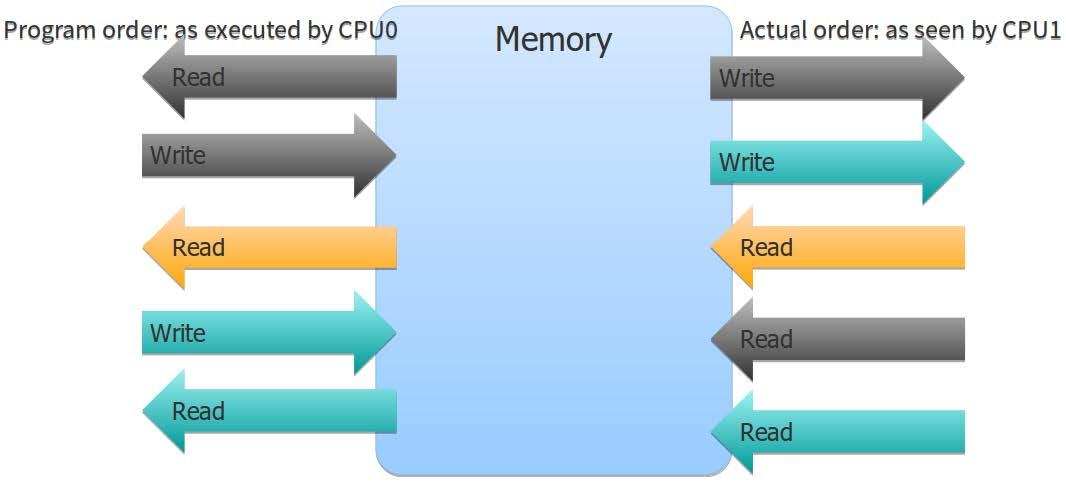
\includegraphics[width=0.9\textwidth]{content/1/chapter5/images/9.jpg}\\
图5.9 - 自由内存序操作的可见性
\end{center}

这就是我们之前讨论过的可见性:一个CPU按照一定的顺序执行操作,但结果对其他CPU是可见的,顺序却不同。为简单起见,我们通常只讨论操作的可见性,而不是每次的结果。

在共享计数器\texttt{N}上的操作是按照自由内存序执行的,这会让我们陷入严重的麻烦中:使程序正确的唯一方法是锁定它,以便只有一个线程(生产者或消费者)运行,并且没有从并发性方面得到性能的改进。

幸运的是,我们还可以使用其他的内存序,比如获取-释放内存序。当原子操作按照这个顺序执行时,可以保证访问内存,并在原子操作之前执行的操作,在另一个线程对同一原子变量执行原子操作之前是可见的。类似地,在原子操作之后执行的操作只有在对同一变量进行原子操作之后才可见。同样,当我们讨论操作的可见性时,是说结果对其他CPU可见。这在图5.10中很明显:在左边,CPU0在执行的操作。在右边,与CPU1看到的相同的操作。特别要注意的是,右边有显式的原子写操作。但是CPU1不执行原子写,它执行一个原子读来查看CPU0执行的原子写的结果。所有其他操作也一样:左边,是CPU0的执行顺序。右边,是CPU1可见的顺序。

%\hspace*{\fill} \\ %插入空行
\begin{center}
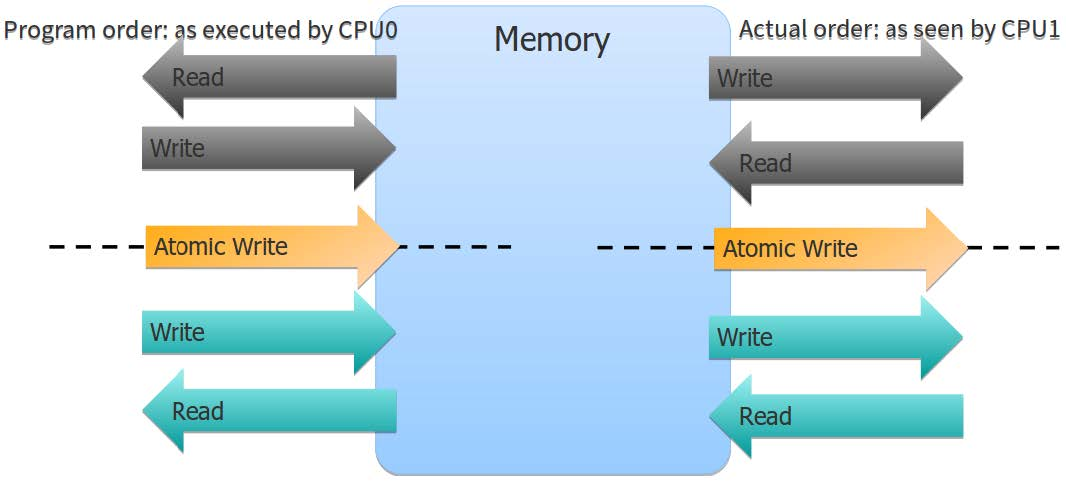
\includegraphics[width=0.9\textwidth]{content/1/chapter5/images/10.jpg}\\
图5.10 - 获取-释放内存序操作的可见性
\end{center}

获取-释放保证是一个包含许多重要信息的简短声明,这里我们来详细阐述几个不同的观点。首先,顺序是相对于两个线程在同一个原子变量上执行的操作定义的。除非两个线程以原子的方式访问同一个变量,否则它们的时钟对彼此来说完全没意义,我们无法推断出在其他事情之前或之后发生了什么。只有当一个线程观察到另一个线程执行的原子操作的结果时,我们才可以在此基础上,对操作之前和之后的行为进行讨论。在生产者-消费者的例子中,生产者以原子的方式增加计数器\texttt{N}。消费者以原子的方式读取同一个计数器。如果计数器没有改变,则对生产者的状态一无所知。但当消费者看到计数器从N变成了N+1,并且两个线程都使用了获取-释放内存序,我们就知道生产者在计数器增加之前执行的所有操作,现在对消费者是可见的。这些操作包括构造相应的元素,并将其保存在数组\texttt{buffer[N]}中所需的所有工作,所以消费者可以安全地进行访问。

第二个要点是,在访问原子变量时,两个线程都必须使用获取-释放内存序。如果生产者使用这个顺序来增加计数值,但是消费者使用自由内存序来读取它,就不能保证操作的可见性了。

最后一点是,所有的顺序都是根据对原子变量的操作之前和之后给出的。同样,在生产者-消费者的例子中,我们知道生产者为构造第N个对象而执行的操作结果,在消费者看到计数器变化时都是可见的。这些操作的可见顺序没有保证,可以在图5.10中看到这一点。当然,这对我们来说并不重要:在构建对象之前,我们不能访问,而当构建完成,我们就不关心完成的顺序了。具有内存序的原子操作保证充当其他操作无法跨越的栅栏,可以在图5.10中想象这样存在这样一个栅栏,它把整个程序分成两个不同的部分:计数之前发生的和计数之后发生的操作。由于这个原因,讨论类似内存栅栏这样的原子操作通常会比较简单。

让我们暂时假设,程序中计数器\texttt{N}上的所有原子操作都有获取-释放栅栏,这肯定能保证程序的正确性。然而,请注意,获取-释放对于我们的需求来说过度了。对于生产者来说,它给了我们保证,当消费者看到计数器从N到N+1的变化时,所有在计数增加到N+1之前构建的\texttt{buffer[0]}到\texttt{buffer[N]}都是可见的。我们需要这样的保证。还可以保证,为构造剩余的对象、\texttt{buffer[N+1]}或更大的对象而执行的操作中,没有一个是可见的。我们不关心这个:消费者不会访问这些对象,直到它看到计数器的更新。在消费者端,我们保证在消费者看到计数器改变为N+1后,执行的所有操作都会在原子操作之后产生效果(内存访问)。我们需要这样的保证:不希望CPU重新排序消费者操作,并在准备好之前执行一些访问对象\texttt{buffer[N]}的指令。但是我们也可以保证消费者处理之前的对象(比如\texttt{buffer[N-1]})所做的工作已经完成,并且在消费者处理到下一个对象之前对所有线程可见。再说一遍,我们不需要这种保证,没有任何操作需要这个保证。

严格的内存序是否有害?对正确性而言,没有。但这是一本关于编写快速程序(也是正确的程序)的书。为什么内存序的保证是必须的呢?因为当让编译器和处理器自己处理时,它们可以以重新排列程序的指令。为什么要这么做呢?通常是为了提高性能。因此,我们对重新排序执行的能力施加的限制越多,对性能的不利影响就越大。因此,我们希望使用的内存序对程序的正确性有足够的限制,但不能太严格。

为生产者-消费者程序提供所需要的内存序如下。在生产者端,我们需要获得-释放内存栅栏所提供的一半保证:所有在使用栅栏的原子操作之前执行的操作,必须在其他线程执行相应的原子操作之前可见。这就是释放内存序:

%\hspace*{\fill} \\ %插入空行
\begin{center}
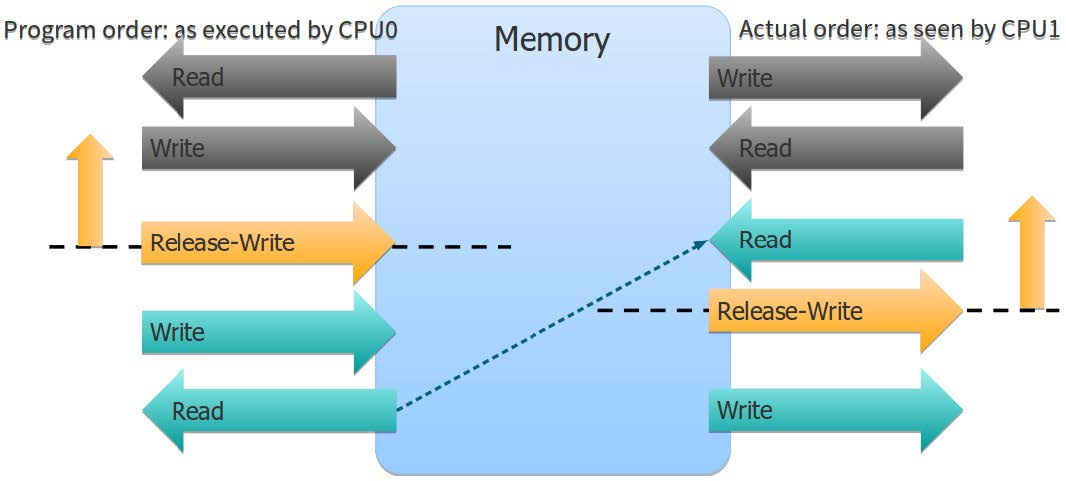
\includegraphics[width=0.8\textwidth]{content/1/chapter5/images/11.jpg}\\
图5.11 - 释放内存序
\end{center}

当CPU1看到CPU0以释放内存序执行的原子写操作的结果时,可以保证CPU1看到的内存状态已经反映给CPU0在这个原子操作之前执行的所有操作。注意,我们没有提到CPU0在原子操作之后执行的操作。正如在图5.11中看到的,这些操作可以以任何顺序显示。由原子操作创建的内存栅栏只在一个方向上有效:在栅栏之前执行的操作都不能跨越它,并且在栅栏之后才看到。但是在另一个方向上,栅栏是可渗透的。出于这个原因,释放内存栅栏和相应的获取内存栅栏有时称为\textbf{半栅栏}。

获取内存序是在消费者端使用的,确保栅栏后执行的所有操作对栅栏后的其他线程可见,如图5.12所示:

%\hspace*{\fill} \\ %插入空行
\begin{center}
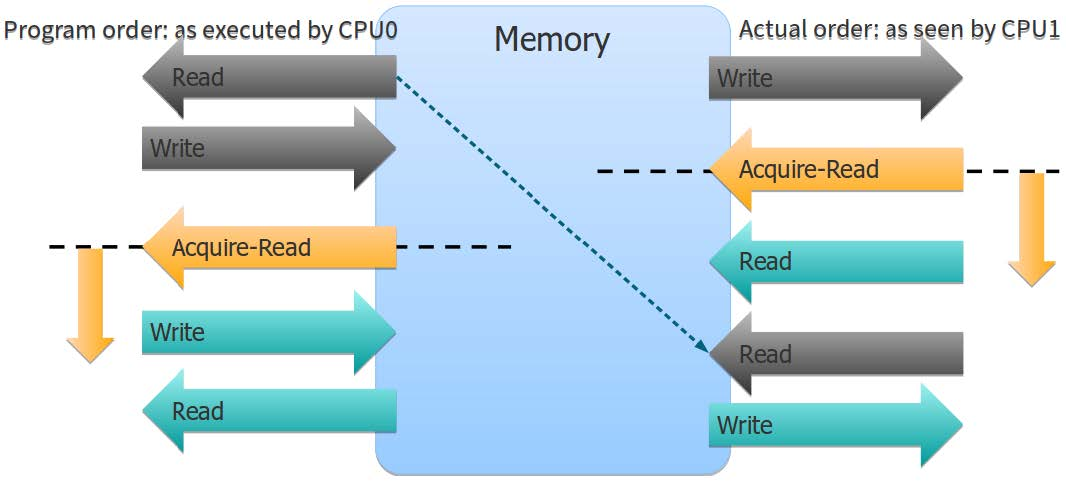
\includegraphics[width=0.8\textwidth]{content/1/chapter5/images/12.jpg}\\
图5.12 - 获取内存序
\end{center}

获取和释放内存栅栏总是成对使用:如果一个线程(在我们的例子中,是生产者线程)使用一个原子操作来释放内存,那么另一个线程(消费者线程)必须在同一个原子变量上使用获取内存序。为什么需要两个栅栏?一方面,可以保证生产者在增加计数之前构建新对象所做的一切,只要看到这个增量,消费者就可以看到。但这还不够,因此需要保证消费者为处理这个新对象而执行的操作不会在时间上向后移动,回到栅栏之前的某个时刻,此时他们可能已经看到了处于未完成状态的对象。

我们知道仅仅对共享数据进行原子化操作是不够的,您可能会问,上面的方法对生产者-消费者项目是否真的有效。事实证明,锁和无锁版本都是正确的,尽管我们没有明确地说明内存序。那么,C++是如何控制内存序的呢?

\subsubsubsection{5.5.3\hspace{0.2cm}C++中的内存序}

首先,让我们回想一下我们的生产者-消费者程序的无锁版本,那个有原子计数器的版本:

\begin{lstlisting}[style=styleCXX]
std::atomic<size_t> N; // Count of initialized objects
T* buffer; // Only [0]…[N-1] are initialized
… Producer …
{
	new (buffer + N) T( … arguments … );
	++N; // Atomic, no need for locks
}
… Consumer …
for (size_t i = 0; keep_consuming(); ++i) {
	while (N <= i) {}; // Atomic read
	consume(buffer[i]);
}
\end{lstlisting}

计数器\texttt{N}是一个原子变量,由模板\texttt{std::atomic}生成的类型对象,类型参数为\texttt{size\_t}。所有原子类型都支持原子读写操作,也就是说,它们可以出现在赋值操作中。此外,整数原子具有以原子方式定义和实现的常规整数操作,因此\texttt{++N}是一个原子增量(并不是所有操作都定义了,例如:没有\texttt{operator *=})。这些操作都没有明确指定内存序,那么我们如何保证内存序呢?实际上,在默认情况下,我们内存序会得到了最严格的保证,即每个原子操作的双向内存栅栏(实际的保证甚至更加严格,您将在下一节中看到)。这就是我们的程序正确的原因。

若认为这有些过度了,那可以将内存序改为所需要的,但必须显式地说明。原子操作也可以通过调用\texttt{std::atomic}类型的成员函数来执行,在这里也可以指定内存顺序。用户线程需要使用获取栅栏进行加载操作:

\begin{lstlisting}[style=styleCXX]
while (N.load(std::memory_order_acquire) <= i);
\end{lstlisting}

生产者线程需要一个带有释放屏障的自增操作(就像自增操作符一样,成员函数也会返回自增操作完成之前的值):

\begin{lstlisting}[style=styleCXX]
N.fetch_add(1, std::memory_order_release);
\end{lstlisting}

我们必须意识到,在优化过程中,已经跳过了一个非常重要的步骤。开始前一段的正确方式是,如果认为这有些过度了,那么必须通过性能测试来证明,只有这样才能将保证达到性能和正确性的真正平衡。即使在使用锁的情况下,并发程序也很难编写,必须证明无锁代码和内存序的正确性。

说到锁,它们内存顺序是什么呢?我们知道,锁保护的操作都将被随后获得锁的任何其他线程看到,但是剩下的内存呢?使用锁所强制的内存序如图5.13所示:

%\hspace*{\fill} \\ %插入空行
\begin{center}
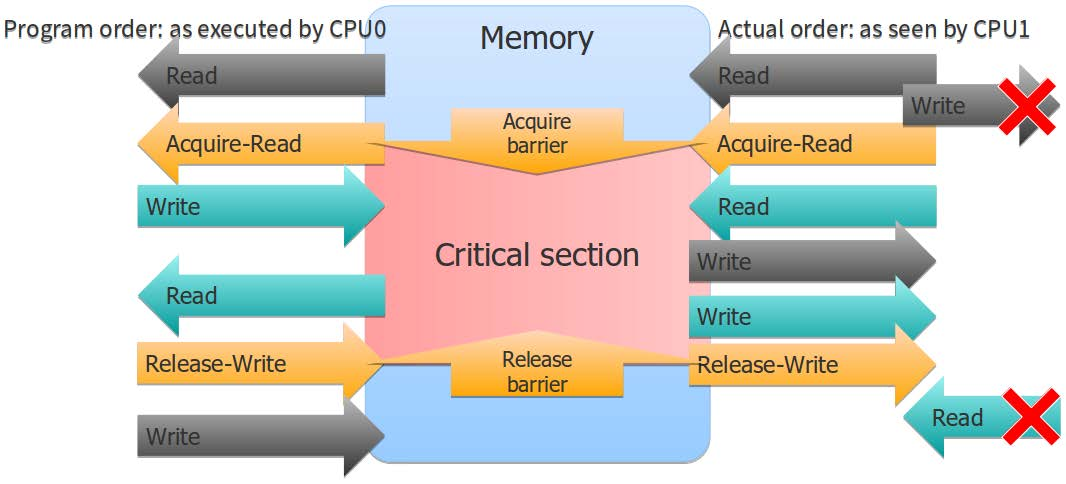
\includegraphics[width=0.9\textwidth]{content/1/chapter5/images/13.jpg}\\
图5.13 - 互斥锁的内存序
\end{center}

互斥对象内部(至少)有两个原子操作。锁定互斥锁相当于读取操作和获取内存序(这解释了名称:这是获取锁时使用的内存序)。任何在栅栏前执行的操作,都可以在越过栅栏后看到,但是任何在获得锁之后执行的操作都不能在之前看到。当我们解锁或释放锁时,即为释放内存序。在栅栏之前执行的操作将在栅栏之前可见,获取和释放这对栅栏充当了夹在它们之间的边界,这就是所谓的临界区:任何在临界区内执行的操作,也就是说,在线程持有锁时执行的操作,在进入临界区时对其他线程都是可见的。任何操作都不能离开临界区(在之前或之后变得可见),但是外部的操作可以进入临界区。至关重要的是,没有这样的操作可以跨越临界区:如果外部操作进入临界区,就不能离开。因此,CPU0在进入临界区之前所做的任何事情,都会在离开临界区之后让CPU1可见。

对于我们的生产者-消费者计划,这转化为以下保证:

\begin{lstlisting}[style=styleCXX]
… Producer …
new (buffer + N) T( … arguments … );
{ // Critical section start – acquire lock
	std::lock_guard l(mN);
	++N;
} // Critical section end - Release lock
… Consumer …
{ // Critical section – acquire lock
std::lock_guard l(mN);
n = N;
} // Critical section – release lock
consume(buffer[N]);
\end{lstlisting}

生产者为构造第N个对象而执行的所有操作,都在生产者进入临界区之前完成。它们将在消费者离开临界区,并开始使用第N个对象之前对其可见。因此,程序是正确的。

刚才阅读的部分介绍了内存序的概念,并举例说明了它。但是,当试图在代码中使用这些知识时,会发现结果非常不一致。为了更好地理解性能,应该从同步多线程和避免数据竞争的不同方法中期望得到什么,所以我们需要一种稍微复杂的方式来描述内存序和相关概念。




































